\chapter{Variational Greedy InfoMax} \label{cha:3}

\section{Motivations} %\section{Problem setting}
	In the previous chapter, we discussed two frameworks of deep representation learning. First, we discussed the autoencoder and its variational counterpart, which minimise the reconstruction error. Secondly, we discussed Contrastive Predictive Coding (CPC) and Greedy InfoMax (GIM), both of which optimise the InfoNCE objective. These two approaches seek to maximise the mutual information between the encodings of data patches that are temporally nearby. The latent representations obtained from all four methods can then be utilised for downstream tasks \citep{bengioRepresentationLearningReview2013a, weiRecentAdvancesVariational2021, oordRepresentationLearningContrastive2019, lowePuttingEndEndtoEnd2020a}
	
	% repr learn autoenc + vae (disentenglement)
		The autoencoder's sole objective is to learn lower dimensional representations of which the original data can be reconstructed. As a result, the representations may serve well for data compression, but no additional constraints are enforced, such as feature disentanglement and thus the latent space may still be hard to work with for downstream tasks \citep{tschannenRecentAdvancesAutoencoderBased2018}. Meanwhile, VAEs with a standard normal prior, enforce representations which break down or disentangle each feature into a narrowly defined variable and encode them as separate dimensions \citep{weiRecentAdvancesVariational2021}. This additional constraint could potentially result in better-suited representations for downstream tasks. To understand why, consider for instance a classifier which is tasked to predict the pronounced syllables corresponding to the latent representation of a speech wave. It would then be beneficial to have all syllable-related information encoded in specific dimensions, which are not influenced by other audio properties, such as the speaker's identity.
	

	% cpc contrasts noise -> smaller architect
		Both autoencoders and VAEs assess the quality of their representations by comparing the original data with its reconstruction. Consequently, their architectures require an additional decoder block, which must also fit into memory. This can be a disadvantage for resource-constrained devices, as the overhead from the decoder restricts the architectures that these devices can train. Meanwhile, CPC and V-GIM learn representations without having to reconstruct the original data. As a result, they do not require a decoder and can benefit from a simplified architecture, while, maintaining state-of-the-art performance \citep{stackeEvaluationContrastivePredictive2020}. A second benefit of CPC and GIM is that they are directly compatible with sequential data.
		
		
	% lead to interpretabil
		Both frameworks (reconstruction and information maximisation algorithms) possess the ability to obtain useful representations for various downstream tasks. However, the content of these representations may not always be intuitive to humans and their structure may be difficult to comprehend. While CPC and GIM are considered state-of-the-art, their performance comes at a cost of having the least interpretable representations. Autoencoders maintain interpretability because a decoder can be used to reveal the information contained in the latent representation. The same transparency can also be achieved with VAEs. Additionally, by using a standard Gaussian as a prior and constraining the latent distributions to be similar to this prior, we can interpolate between representations and observe the effects through the decoder. As such, we can observe the specific information that is contained in each of the representation's components (channels in ConvNets or neurons in fully connected ANNs). VAEs can also result in disentangled features, further enhancing interpretability \citep{grossuttiDeepLearningInfrared2022}. In contrast, CPC and GIM do not contain a built-in decoder mechanism, nor pose constraints on the latent space, significantly reducing interpretability.
		


\section{Towards Decoupled Training for Probabilistic Representations} \label{cha:vgim_decoupled_training_for_probabil_repr}
	% Our contribution
		In what follows next we introduce Variational Greedy InfoMax (V-GIM), maintaining the state-of-the-art performance obtained from optimising the InfoNCE objective, while leveraging the interpretable and disentangled benefits from VAEs. This is achieved by optimising a novel loss function, \textit{Variational-InfoNCE}, a combination of InfoNCE and the regularisation term from VAEs. Additionally, by splitting up the neural network into modules, as introduced in \citep{lowePuttingEndEndtoEnd2020a}, we greedily optimise each module with its own instance of this loss function. As a result, the interpretability benefits from VAEs will also be applicable in-between modules. This is in contrast to VAEs where solely the final output representations are interpretable.		
				
	% How:
		% still maximise mutual information between zt, ztk, but predictions no longer fixed datapoints.
		% xt -> cpc model -> q( . | xt) = mui, sigmai
		
		As discussed in the section on CPC, a patch of sequential data $\xt$ is encoded through $g_{enc}(\xt) = \zt$ and aggregated over previous encodings through auto-regressor $g_{ar}(\z_1  \dots \zt) = \ct$, where both $\zt$ or $\ct$ may serve as representations for downstream tasks. The encoder function $\genc$ is usually represented by a ConvNet, and $\gar$ by a Gated Recurrent Unit (GRU).
		Finally, the encoding functions $\genc$ and $\gar$ are obtained by optimising a global loss function, the InfoNCE loss, end-to-end via backpropagation. 

		% split in modules
			Instead, in this study, we split up $\genc$'s network architecture by depth into $M$ modules 
			$$g_{enc}^1(\cdot),~ g_{enc}^2(\cdot),~\dots,~g_{enc}^M(\cdot)$$ 
			and prevent gradients from flowing between modules, as introduced in GIM. An additional optional $M \! + \! 1$'th module $\gar$ can be appended to the architecture. Each module is greedily optimised via a novel loss function, $\Lvnce$, which we will define in section \ref{cha:vgim_learning_objective}. Each module's output serves as input for the successive module, as presented in the following equations. %#, and depicted in figure \ref{fig:variationalgim}.			
				%			\begin{figure} % fig: overview multiple modules
				%				\centering
				%				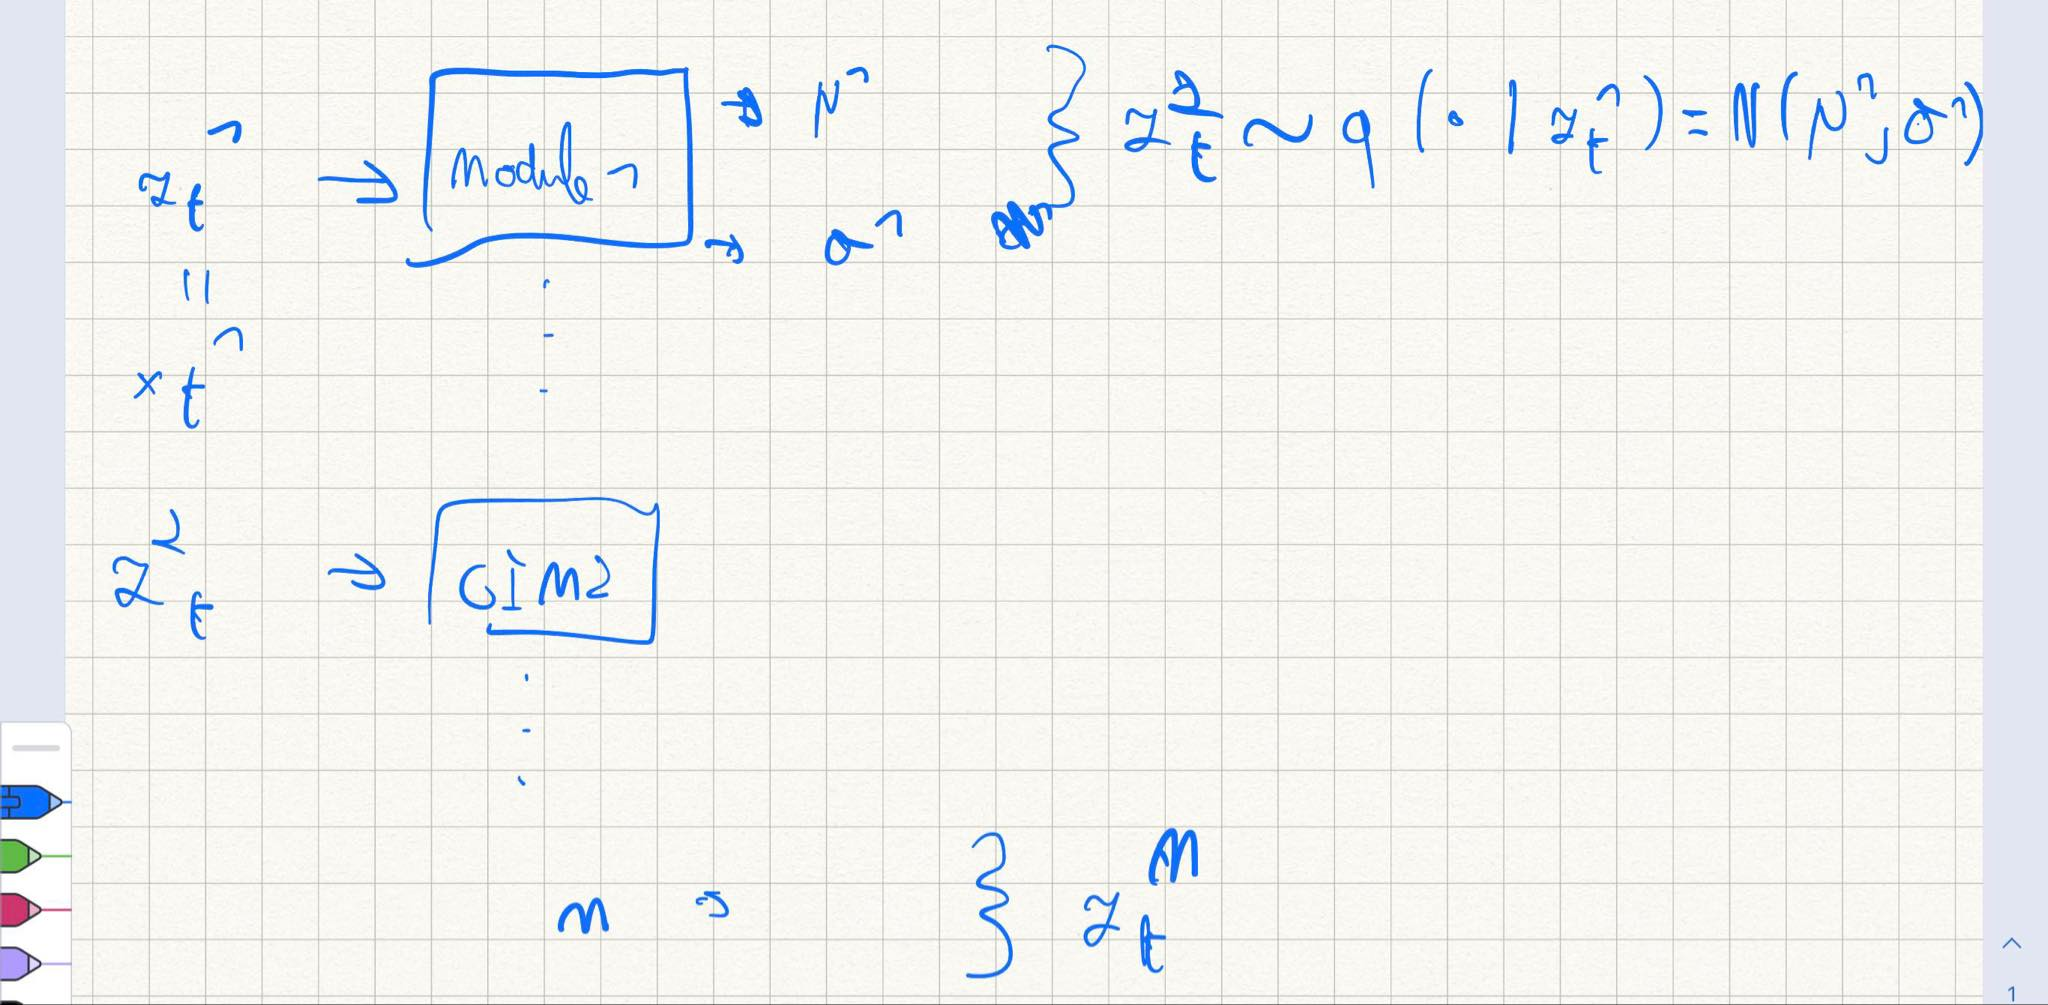
\includegraphics[width=0.7\linewidth]{temp_variational_gim}
				%				\caption{}
				%				\label{fig:variationalgim}
				%			\end{figure}
			\begin{align*} % g_enc1, ...
				g_{enc}^1(\xt) &= \zt^1 \\
				g_{enc}^m(\zt^{m-1}) &= \zt^m \\
				g_{ar}(\z_1^M ~ \dots ~ \zt^M) &= \ct
			\end{align*}
			
			The final representation $\zt^M$ is obtained by propagating $\xt$ through each modules as follows:
			$$ g_{enc}^M ( \dots	g_{enc}^2(g_{enc}^1(\xt))) = \zt^M$$
			
			% TODO: WANNEER OVER GRADIENTS BEGINT, A SINGLE MODULE IS DEFINED AS FOLLOWS.. MET F(z m-1) -> (mu, sigm)
			
			
					
		% Distributions
			Additionally, taking inspiration from VAEs, the outputs from $\gencm$ and $\gar$ are in fact samples from a distribution denoted by $q(\zt^m \mid \zt^{m-1})$, defined as a multivariate Gaussian with diagonal covariance matrix, as follows:
			\begin{equation}
				\sampleqdot{\zt^{m-1}} = \normalfatmusigma \label{eq:def_q_vgim}
			\end{equation}
			with $\mufat$ and $\sigmafat$ dependent on $\zt^{m-1}$.
			The outputs for $\gencm$ and $\gar$ are obtained by sampling from this distribution, denoted respectively, as follows:
 			\begin{align} % z ~ q AND c ~ q
			 	\sample{\zt^m}~ & \qfromzmneg  \label{eq:sample_z_from_q} \\
			 	\sample{\ct}~ & \qfromzM
			 \end{align}
			We call these distributions the \textit{posterior} distributions. Modules are thus stochastic and computing $g_{enc}^m(\zt^{m-1})$ twice will likely result in two different representations of $\zt^m$. This is in contrast to CPC and GIM's latent representations which remain fixed depending on the input \citep{oordRepresentationLearningContrastive2019, lowePuttingEndEndtoEnd2020a}.
		
		% How distributions: predict q + sample
			We achieve these stochastic modules by defining each module $\gencm$ consisting of two blocks. The first block receives as input $\zt^{m-1}$ and predicts the parameters $\mufat$ and $\sigmafat$, which fully describe the distribution $\qfromzmneg$ defined in equation \ref{eq:def_q_vgim}. The second block samples $\sample{\zt^m} \sampleqmdot{\zt^{m-1}}$ from this distribution and produces an output representation. This is depicted in figure \ref{fig:single_variational_module}.
			
						
\begin{figure}[h]
	\centering
	\tikzstyle{arrow} = [thick,->,>=stealth]
	\begin{tikzpicture}[
		AnnNode/.style={trapezium, draw=black,
			trapezium stretches=true,
			minimum width=2cm, 
			minimum height=1.5cm,
			rotate=-90,
			trapezium angle=75,
			very thick},
		SamplingBlock/.style={rectangle, draw=black,
			minimum height=1cm, minimum width=2cm,
			very thick},
		]
		
		\node[AnnNode] (enc) {\rotatebox{90}{ANN}};
		\node[SamplingBlock] [right of=enc, xshift=2.5cm] (sample) {$\zt^m \sim \sampleqdot{\zt^{m-1}}$};
		
		% enc edges
		\draw[->] ++(-2.5, 0) -- (enc.south) node[above, midway] {$\zt^{m-1}$};
		\draw[->] 
		[transform canvas={yshift=.7em}] 
		(enc.north) -- (sample.west) node[above, midway] {$\mufat$};
		
		\draw[->] 
		[transform canvas={yshift=-.7em}] 
		(enc.north) --  (sample.west) node[below, midway] {$\sigmafat$};
		
		\draw[->] 
		(sample.east) --  ++(1.5, 0) node[above, midway] {$\zt^m$};
		
		
		
		
	\end{tikzpicture}
	\caption{A single module.}
	\label{fig:single_variational_module}
\end{figure}

			
		% define ztm~q() = gaussian., --> z = mu + sigma*noise
			In practice, sampling from $q^m$ is achieved through a reparametrisation trick, as introduced in \citep{kingmaAutoEncodingVariationalBayes2022}. The equation to compute $\zt^m$ then becomes:
			\begin{equation*}
				\zt^m = \mufat + \sigmafat \odot \epilonfat
			\end{equation*}
			where $\epilonfat$ corresponds to a sampled value $\samplestandardnormal{\epilonfat}$ and $\odot$ is element-wise multiplication. The procedure to obtain $\ct$ is analogous to $\zt^m$.
			
	
		
\section{The Loss Function} \label{cha:vgim_learning_objective}
	Instead of training the neural network's modules end-to-end with a global loss function, each module is optimised greedily with its own personal loss function. Through the introduction of the novel \textit{Variational-InfoNCE} loss, mutual information between temporally nearby representations is maximised, while regularising the latent space to be approximate to the standard Gaussian $\standardnormal$. The Variational-InfoNCE loss is defined as follows:
	
	\begin{equation} % variational_gim_loss % TODO: die k's is niet echt correct/onvolledig
		% \mathcal{L}(\ztk^{m-1}, \zt^{m-1}) = 
		\Lvnce^m =
		\underbrace{\reconstrgim}_{\text{Maximise } I(\ztk^m, \zt^m)} + \underbrace{\beta ~ \latentspaceconstraintgim}_{\text{Regularisation}}
		\label{eq:variational_gim_loss}
	\end{equation}

	Here, $m \in \naturalset$ refers to the $m$'th module and $k \in \naturalset$ the number of patches in the future the similarity score $\fkm$ must rate. The latent representations $\ztk^m$ and $\zt^m$ are encoded samples produced by $g_{enc}^m(\ztk^{m-1})$ and $g_{enc}^m(\zt^{m-1})$, respectively and $X$ is a set of samples ${ \left\{ \ztk^m, \z_1^m, \z_2^m, \dots \right\} }$ where $\zj^m$ with $j \neq t \! + \! k$ are random samples.


	The similarity score $f_k^m(\cdot)$'s definition is identical to \citep{lowePuttingEndEndtoEnd2020a}:
	
	$$ f_k^m(\ztk^m,\zt^m) = \exp({\ztk^m}^TW_k^m\zt^m) $$
	
	
	$\Lvnce^m$ consists of two terms. The first term ensures that latent representations of temporally nearby patches contain maximised mutual information. The second pushes the latent representations close to the origin. Finally, $\beta$ is a hyper-parameter which decides the relative importance between the two terms. $\beta >> 1$ will weight more importance to regularisation but may result in posterior collapse \citep{lucasUnderstandingPosteriorCollapse2022}. On the other hand, $\beta \approx 0$ will put more importance to the mutual information maximisation term while forgetting about the regularisation term. When $\beta = 0$, V-GIM is identical to GIM but with an altered neural network architecture which supports probabilistic latent representations.
	% TODO: IK KAN NOG PARAGRAAF TOEVOEGEN OVER MI MAXIM, DE LOWERBOUND: UITBREIDING + MI(X, Z) maar ook MI(zt, zt+k).
	
	\subsection{The Gradient}
%		Similar, to VAEs \citep{kingmaAutoEncodingVariationalBayes2022}, 
		To estimate the expectation term in $\Lvnce$, we apply the same approximation method as in VAEs, achieved through Monte Carlo estimates \citep{kingmaAutoEncodingVariationalBayes2022}. The first term $\Lvnce$ in then becomes:
		\begin{align*}
			\reconstrgimMontecarlo 	
		\end{align*}
		Here, $L$ refers to the number of samples drawn for a single data point and each ${\ztk^m}^{(l)}$ or ${\zt^m}^{(l)}$ is a different sample. However, as argued by Kingma and Welling, choosing a large batch size will allow this value to be set to 1 without harming performance \citep{kingmaAutoEncodingVariationalBayes2022}.
		
		With regards to the second term, since $\qfromzmneg$ is a Gaussian defined by parameters $\mufat$ and $\sigmafat$, a closed-form solution exists \citep{kingmaAutoEncodingVariationalBayes2022}. The closed form equation is the following:
		\begin{equation*}
			\latentspaceconstraintgim = \latentspaceconstraintclosedformNoI
		\end{equation*}
		Therefore, this term can be directly computed and does not need to be approximated through Monte Carlo. The gradient for the two terms can then be computed using an automatic differentiation tool such as PyTorch \citep{paszkeAutomaticDifferentiationPyTorch2017}.
			
	
	\subsection{Properties of the Latent Space} \label{cha:contin_space}	
	In this section, we present two important conjectures regarding the structure of the latent space defined by each of V-GIM's modules. For each module $\gencm$ (or analogously for $\gar$), an input space $\Z^{m-1}$ is mapped to a latent space $\Z^m$ as follows: 
	$$g_{enc}^m: \Z^{m-1} \rightarrow \Z^m$$
	Here, $\Z^0$ equals the feature space $\X$. The two conjectures hold true when $\Lvnce$ is optimal. They will serve as the main argument for why V-GIM's representations are interpretable, discussed in section \ref{cha:vgim_benefits}. Meanwhile, traditional techniques such as CPC and GIM lack these interpretable benefits.
	
		\subsubsection{Conjecture 1: $\Z^m$ is uninterrupted and well-covered around the origin.}
			In V-GIM, a latent representation $\zt^m \in \Z^m$ of a data point $\zt^{m-1} \in \Z^{m-1}$ is a sample from the Gaussian distribution $q^m(\cdot \mid \zt^{m-1})$. Thus, encoding the same $\zt^{m-1}$ an infinite number of times results in an entire spherical region (around a particular mean $\mufat$) in $\Z^m$ that is entirely covered by the latent representations corresponding to $\zt^{m-1}$, without any interruptions in this region. This is different from GIM and CPC where a data point merely covers a single point of the latent space (and not an entire region). Furthermore, because each region should be close to the origin, regions are more likely to utilise the limited space efficiently around the origin, resulting in a lower chance of obtaining large holes between two regions from different data points. As a result, the latent representations from the dataset should cover the entire latent space around the origin, such that all latent representations around the origin have a corresponding data point that is similar to a data point from the dataset.
		
	
		\subsubsection{Conjecture 2: $\Lvnce$ enforces smooth and consistent transitions in the latent space with respect to the mutual information of the original data points.}
			As we discussed in section \ref{cha:vgim_learning_objective}, the first term in $\Lvnce$ maximises the mutual information $I(\ztm, \ztk^m)$, which was proven by \cite{oordRepresentationLearningContrastive2019}. However, in addition, \cite{lowePuttingEndEndtoEnd2020a} argue that when modules are trained in a greedy setting using this loss function, the mutual information between outputs of successive modules $I(\zt^{m-1}, \zt^{m})$ is also maximised, and therefore also $I(\xt, \zt^{m})$. Or equivalently, given a data point $\xtith$, the output produced by $ g_{enc}^m ( \dots	g_{enc}^2(g_{enc}^1(\xtith))) = \zt^m$ will ensure $I(\xtith, \zt^{m})$ to be maximum. This is an important observation. Now, since the latent representations corresponding to $\xtith$ cover an entire spherical region (as discussed in conjecture 1), the mutual information $I(\xtith, \ztm)$ for all the latent representations $\ztm$ in this region should be maximised.
			
			Let us now consider a second data point $\xtjth$ whose corresponding regions in $\Z^m$ overlap with $\xtith$'s region. Since regions are fairly large and the latent space is small, this is likely to happen. Due to the overlap between the regions, there exists a latent representation ${\ztm}'$ that corresponds to both $\xtith$ and $\xtjth$. 
			Since ${\ztm}'$ is lower dimensional and is defined such that $I({\ztm}', \xtith)$ and $I({\ztm}', \xtjth)$ are both maximised, ${\ztm}'$ contains information that is common to both $\xtith$ and $\xtjth$ (if not, ${\ztm}'$ would not have been in the two regions).
			
			If small changes to the components of ${\ztm}'$ caused abrupt changes in the corresponding feature vectors in $\X$, this would be heavily penalised by $\Lvnce$ due to the width of the Gaussian regions. Therefore, the transitions in the latent space must be smooth to ensure that small changes in ${\ztm}'$ lead to small changes in the corresponding feature vectors in $\X$.
			
			Furthermore, due to the definition of $q^m$ with covariance matrix containing only non-zero values on the diagonal, the components of $q^m$ are independent. Therefore, moving a latent representation in a single direction of a particular dimension should cause the same effect on the mutual information with respect to the corresponding data point in $\X$ as moving it in a different dimension. This property ensures that the transitions in the latent space are consistent.
							
			Finally, the result of these two conjectures is an uninterrupted latent space around the origin 
			where moving a latent representation towards a particular dimension in the latent space causes smooth and consistent changes in the corresponding data point from the previous module's latent space. This crucial observation will serve as the main argument for why V-GIM's representations are interpretable, while traditional techniques such as CPC and GIM do not have these guarantees. 
		
		
			


		
\section{Computational Benefits} \label{cha:vgim_benefits}
	Each module in V-GIM is greedily trained through the variational InfoNCE loss. This approach, as suggested by \cite{lowePuttingEndEndtoEnd2020a}, offers several computational benefits, including decoupled and asynchronous distributed training. Modules can then be trained in parallel on multiple devices, or sequentially on a single device. This is particularly interesting for memory-constrained devices, 
	as it enables the training of architectures that exceed the available memory capacity. Furthermore, V-GIM mitigates the vanishing gradient problem, a well-known issue in deep architectures, by preventing the flow of gradients between modules \citep{huHandlingVanishingGradient2021}.
	
	In addition to the benefits associated with greedy training, V-GIM adds a constraint to the latent space produced by each module, resulting in further practical benefits. Since V-GIM adopts a greedy training approach, these benefits apply not only to the final module's output but also to the outputs of intermediate modules.
	

	\subsubsection{Interpretability of final and intermediate modules}
		By regularising the latent space resulting in the properties discussed in section \ref{cha:contin_space}, each of V-GIM's modules define a space where sampling from a point around the origin is likely to correspond to a data point that is similar to the dataset. A decoder trained on this space will generalise well to unseen data when given a latent representations around the origin. This has significant implications for V-GIM's interpretability. Not only can we assess the information contained in a latent representation through a decoder, but we can also attempt to understand the underlying structure of the latent representation. This is achieved in a similar way as with VAEs, where manipulating a individual dimension's value and observing the effect through the decoder gives insight into the specific information contained in that dimension.
		
		Furthermore, since V-GIM's neural network architecture consists of a variable number of modules, each with its own interpretable latent space, these benefits are applicable to the latent representations produced by intermediate modules, allowing us to observe the internal mechanism of the neural network. Additionally, since convolution layers in ConvNets typically reduce the length of representations, different modules encode different sequence lengths, encouraging different abstractions to be learned at different levels. By having intermediate modules be interpretable, we can analyse these abstractions as well. This is in contrast to VAEs, where only the output latent representation is interpretable, and intermediate representations in the architecture are not.
		
		In contrast, GIM and CPC do not pose constraints on the latent space. Although a decoder can still be trained on the latent representations of GIM and CPC, the latent space is highly unpredictable. Consequently, 
		it is not guaranteed that the reconstructed output from a randomly sampled latent representation will be meaningful, as it may be very dissimilar from the original data. Moreover, attempting to decode an interpolated representation from two existing latent representations may not lead to a meaningful output either, since the latent space the decoder was trained on may contain large gaps. This makes it challenging to interpret the underlying structure of the latent representations defined by CPC and GIM.

						
	\subsubsection{Disentanglement}
		In section \ref{cha:disentang} on $\beta$-VAEs and disentanglement, \cite{higginsBetaVAELearningBasic2022} argue that setting the prior $p(\vect{z})$ to an isotropic Gaussian encourages disentanglement in the encodings. When encodings are fully disentangled, this results in each dimension from the encoding capturing a different property of the original data. Since $\Lvnce$ enforces the latent space to be standard normal, this theorem is also applicable to V-GIM and choosing a large value for $\beta$ in $\Lvnce$ applies more pressure for encodings to be disentangled further increasing interpretability.
		
	
	\subsubsection{Improved generalisation performance through representation variance}
		V-GIM's encodings are samples from a distribution, which means that a single patch of data $\xt$ has multiple encoded representations $\zt^M$. For downstream tasks with little labelled data, the variability in representations could serve as an internal data augmentation method, making the set of plausible decision boundaries smaller, and therefore also improving generalisation to unseen data. This motivation is further depicted in figure \ref{fig:set_of_decision_boundaries} where a two-dimensional latent space and the set of its plausible decision boundaries are shown.
		
		\begin{figure}
			\centering
			\hspace*{1.5cm}
			\begin{annotatedFigure}
				{\includegraphics[width=0.8\linewidth, trim={5cm 4.5cm 0 4cm}, clip]{"graphs/linear boundary"} }	
			\end{annotatedFigure}
			\caption{Example of a two-dimensional space obtained from GIM and V-GIM respectively, where a binary classifier is given three data points. The black lines represent all the possible decision boundaries, while the circular areas in V-GIM represent the samples obtained from the corresponding Gaussian distribution.}
			\label{fig:set_of_decision_boundaries}
		\end{figure}
		
		%Because of this probabilistic approach, a single patch of data $\xt$ will have multiple representations $\zt^M$, providing increased variance in the representations. This can potentially benefit downstream tasks, particularly when labelled data is scarce \citep{weiRecentAdvancesVariational2021}, leading to improved performance. % TODO: this benefit should be moved to benefits section.

	
	\subsubsection{Internal batch normalisation mechanism} \label{cha:vgim_batch_norm}
		During the training of ANNs, the weights of different layers undergo changes, which can lead to a problem known as ``internal covariate shift" \citep{ioffeBatchNormalizationAccelerating2015a}. This shift causes the distributions of each layer's input to change over time, which in turn can negatively affect subsequent layers, slowing down the training process \citep{bjorckUnderstandingBatchNormalization2018, lecunEfficientBackProp1998}. This issue is typically addressed via batch normalisation \citep{santurkarHowDoesBatch2018, bjorckUnderstandingBatchNormalization2018}, a mechanism which normalises the activations of internal layers, allowing for a higher learning rate during training and thus accelerating the process.
			
		Batch normalisation is especially important in a greedy setting such as GIM and V-GIM, where modules are independently trained in parallel. Without intermediate normalisation, subsequent modules may learn slower than previous modules, resulting in the subsequent modules not being able to catch up in time to the changes from preceding modules made during training. The result would be that modules may have to be trained with different learning rates, resulting in an additional hyperparameter that must be obtained for each module.
		% TODO: ^^ maybe in the paragraph is not clear that parallel training means outputs from module1 are given to module2, while both are training, so module 2 learns from inputs that may change later in the future.
		
		In contrast, V-GIM already contains an internal normalisation mechanism in-between modules. This is indirectly caused by regularising each module's latent space to have a zero-mean and standard deviation of one. Finally, the normalised encodings can also be beneficial for downstream tasks. If normalisation is desired, computing the mean and standard deviation over a potentially very large dataset is not required, as this is already built into the encodings.

	
	

	

		% Copy from Higgins: where the KKT multiplier β is the regularisation coefficient that constrains the capacity of the latent information channel z and puts implicit independence pressure on the learnt posterior due to the isotropic nature of the Gaussian prior p(z)





	%	Better generalisation for downstream tasks
%		- Overfitting: reduction of required labelled data needed. Similar data is similar region, the kl divergence makes regions bigger.
%
%		% copied from a bit higher
%		% Because of this probabilistic approach, a single patch of data $\xt$ will have multiple representations $\zt^M$, providing increased variance in the representations. This can potentially benefit downstream tasks, particularly when labelled data in scarce \citep{weiRecentAdvancesVariational2021}, leading to improved performance. % TODO: this benefit should be moved to benefits section.
%
%		Overfitting during inference:
%		- The same datapoint has multiple (similar) representations, such that learning techniques for downstream tasks will not be able to "memorise" the latent space as easily.
%		
%		- Holes: more predictable inference, such that unseen data is more likely to be near clusters. And thus downstream tasks receive latents that are more similar to what is seen before.
%		= better generalisation






%\textbf{Other sources:} \\
%!!! Abstract on VAE: The fundamental idea in VAEs is to learn the
%distribution of data in such a way that new meaningful data with more intra-class variations can be generated
%from the encoded distribution.
%The ability of VAEs to synthesize new data with more representation variance
%at state-of-art levels provides hope that the chronic scarcity of labeled data in the biomedical field can be
%resolved.
%--> and thus for downstream tasks, has a way of obtaining more labelled data? --> better generalisation


%The goal of representation learning is to be useful for downstream tasks. The most important meta-prior is called ‘disentanglement’ which is an unsupervised learning technique that breaks down, or disentangles, each feature into narrowly defined variables and encodes them as separate dimensions 

%Intuitively, a factorial code disentangles the individual elements that were originally mixed in the sample, just as
%humans recognize complex things by disentangling independent elements. If the dimensions of the latent vector are
%independent of each other, it is factorial disentangled, i.e., a
%good representation. VAEs have made such nonlinear latent
%variable models tractable for modeling complex distributions,
%and efficient extraction of relevant biological information
%from learned features for biological data sets, referred to as
%unsupervised representation learning
%https://ieeexplore.ieee.org/stamp/stamp.jsp?tp=&arnumber=9311619








%We show that the Beta-VAE outperforms principal component analysis (PCA) and learns interpretable and independent representations of the generative factors of variance in the spectra %https://pubs.acs.org/doi/pdf/10.1021/acs.jpclett.2c01328
%


